
\section{\acs{DQL} Commands In Depth}
\paragraph{} In this section we will cover the \acf{DQL} commands. The select statement is also called query, because it's responsible for querying the database to read data from it. What we will see here can be applied also to \acs{DML} commands.\\\textbf{Purpose:} Define the structure of the database and its objects.\\\textbf{Auto-Commit:} No.
\subsection{Basic DQL Operations}
\begin{lstlisting}[language=SQL]
-- Content Summary:
-- Single Quotes ' vs Double Quotes "
-- Equal/Not Equal/Greater/Greater or Equal/Less/Less or Equal
-- In/Not In/Is Null/Is Not Null/Like/Not Like/Wildcards/Escape Wildcards and Special Characters
-- And/Or and ()
-- Between/Not Between/Order By (Asc/Desc)
-- Alias
-- Distinct
-- Show Warnings

-- Single Quotes ' vs Double Quotes "
-- The standard supported in all SQL Systems is Single Quotes to define Strings
-- Double Quotes are supported by some DBMS but it's not a standard
select * from book where book_title = 'IT'; -- Standard SQL, supported by all DBMS
select * from book where book_title = "IT"; -- Non Standard SQL, may not work in some DBMS

-- Equal: =
select * from book where book_language = 'Italian';
-- Not Equal: <>
select * from book where book_language <> 'English';

-- Greater: >
select * from book where release_year > 2009;
-- Greater or Equal: >=
select * from book where release_year >= 2009;
-- Less: <
select * from book where release_year < 1521;
-- Less or Equal: <=
select * from book where release_year <= 1521;

-- In: in (value1, value2, ....)
select * from book where book_language in ('German', 'French');
-- Not In: not in (value1, value2, ....)
select * from book where book_language not in ('English', 'German');

-- Is Null: is null (= null is not working)
select * from author where deathday is null;
-- Is Not Null: is not null (<> null is not working)
select * from author where deathday is not null;

-- Like:
select * from author where first_name like 'Da%'; -- match 0 or any number of any characters
select * from author where first_name like 'Da_'; -- match exactly one any character
-- Not Like:
select * from author where first_name not like 'D%';

-- Wildcards:
-- %: match with 0 or any number of any character
-- _: match with exactly one any character
-- wildcards act as wildcards only with like/not like, not with = or <>

-- Escape wildcards/Special Characters:
select * from book where title like '%Handmaid\'s%';
-- Use \ before any wildcard/special character if you want sql to treat it as normal character

-- And/Or
select * from author where first_name like 'Da%' and first_name not like 'Da_';
select * from author where first_name like 'Da%' or first_name like 'Sa%';

-- Use of () to specify the priority of logical operations with and/or
-- If no () is used, SQL will apply the conditions from left to write

-- Example:
select * from author where (first_name like 'Da%' or first_name like 'Sa%') and birthday like '19%'; -- 2 rows
select * from author where first_name like 'Da%' or first_name like 'Sa%' and birthday like '19%'; -- 3 rows
-- why second query gives one more row? because SQL executes the operations from left to write so it's equivalent to below
select * from author where first_name like 'Da%' or (first_name like 'Sa%' and birthday like '19%'); -- 3 rows
-- so the condition and birthday like '19%' is applied only for names that start with Sa

-- Between
select * from book where release_year >= 1950 and release_year <= 1955; -- 3 rows
-- Between is the alternative equivalent for the above
select * from book where release_year between 1950 and 1955; -- 3 rows
-- notice in above case years 1950 and 1955 are included

-- Not Between
select * from book where release_year < 1321 or release_year > 2016; -- 2 rows
-- Not Between is the alternative equivalent for the above
select * from book where release_year not between 1321 and 2016; -- 2 rows
-- notice in this case however 1321 and 2016 are not included

-- Order By Asc/Desc - default: Asc
select * from book order by release_year; -- order by release year in (default) ascending order
select * from book order by release_year asc; -- same as above
select * from book order by release_year desc; -- same but in descending order now

-- Alias
-- Syntax: select <t.columnA as alias_for_columnA>, <t.columnB columnBAlias> from <table as t>;
-- Example:
select a.first_name as author_first_name, a.last_name author_last_name from author as a;

-- Distinct
select last_name, count(*) from author group by last_name having count(*) > 1; -- notice Bronte name exists twice

select last_name from author; -- 21 rows
select distinct last_name from author; -- 20 rows
-- Why? Because if same value exists twice in db, it will only show once with distinct - in this case it's Bronte

-- Show Warnings: To see details of latest error
select 1/0; -- try division by 0 to see warnings
show warnings;
\end{lstlisting}
\subsection{Types of Joins}
\paragraph{} Joins in \acs{SQL} is a very important part. When you need to access data from the database usually you need to combine the results from more than one tables, joins is the tool that gives as this ability in a few different ways. There are four types of joins:
\begin{itemize}
	\item \textbf{(Inner) Join:} Returns the rows that match in both tables.
	\item \textbf{Left (Outer) Join:} Returns all the rows from the left table, and the matched rows from the right table.
	\item \textbf{Right (Outer) Join:} Returns all the rows from the right table, and the matched rows from the left table.
	\item \textbf{Full (Outer) Join:} Returns all the rows that match either the left or the right table.
\end{itemize}
\begin{figure}[h]
	\centering
	\subfloat[\centering Figure: Types of Joins]{{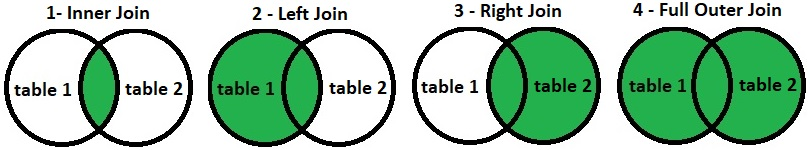
\includegraphics[width=15cm]{types-of-joins}}}
\end{figure}
\begin{lstlisting}[language=SQL]
-- Contents: Comma, (Inner) Join, Left (Outer) Join, Right (Outer) Join,, FUll (Outer) Join, Cross Join

-- Comma
select	*
from	author a, book b
where	a.author_id = b.author_id
; -- 67 results - but we have 69 books? (because 2 books have null author_id)

-- (Inner) Join
select	*
from	author a
join	book b -- or replace with equivalent: inner join
on		a.author_id = b.author_id
; -- again 67 same results
-- Join will shows all results that exist both in left (author) and right (book) table
-- In simple words in this case it produces a table with all authors who have at least one book and their books

-- Left (Outer) Join
select		*
from		author a
left join	book b -- or replace with equivalent: left outer join
on			a.author_id = b.author_id
; -- now 68 results
-- Why? Left Join shows all results of the left (author) table, even if there is no match in right (book) table
-- Notice Virginia Woolf appears in results and book columns are populated with null, since she has no book associated with her
-- In simple words in this case it produces a table with all authors even if they don't have any book and their books

-- Right (Outer) Join
select		*
from		author a
right join	book b -- or replace with equivalent: right outer join
on			a.author_id = b.author_id
; -- now 69 results
-- Why? Right Join shows all results of the right (book) table, even if there is no match in left (author) table
-- Notice books 'The SQL Cook Book' and 'Novel Nook Murders' have no author details, because we didn't associate them with any author

-- Full Join - MySQL doesn't support Full Join
-- How can it be achieved?
select		*
from		author a1
left join	book b1
on			a1.author_id = b1.author_id
union
select		*
from		author a2
right join	book b2
on			a2.author_id = b2.author_id
; -- now 70 results
-- Why? Full Join shows all results of the left (author) and the right (book) table, even if there is no match in the other table
-- Notice now books 'The SQL Cook Book' and 'Novel Nook Murders' and author Virginia Woolf show in results even though they have no much
-- Note: Union combines the results returned by two queries, we will see it better later

-- Cross Join (Cartesian Join)
select		*
from		author a
cross join	book b
; -- 1449 results
-- Why? Cross Join will match every row from table left table, with every row from table right table
-- This kind of join is rarely used

-- Note: Difference between Join and Cross Join is that on Join we should use on to define how rows will be matched from one table with the other ones while Cross Join there should be no on conditions
-- Some DBMS like MySQL allow (Inner) Join without on condition and Cross Join with on
\end{lstlisting}
\subsection{Union/Union All/Intersect/Minus}
\begin{itemize}
	\item \textbf{Union:} returns the joined result set of two or more selects, distinct values only.
	\item \textbf{Union All:} returns the joined result set of two or more selects, allows duplicates.
	\item \textbf{Intersect:} returns the common distinct rows of two or more selects.
	\item \textbf{Minus:} returns the result set that exists on first select, but not on the second select .
\end{itemize}
\begin{lstlisting}[language=SQL]
-- Contents: Union/Union Al/Intersect/Minus

-- Union/Union All
-- Union operator is used to join the result set of two or more select statements
-- The data all selects under union return must have same structure (number of columns, order and similar data types)
-- Union vs Union All: Union selects distinct values while union all allows duplicates
create table tmp_numbers_a (num_x int, num_y int);
create table tmp_numbers_b (num_k int, num_l int);
insert into tmp_numbers_a values (1, 2), (2, 3), (3, 4), (4, 5), (1, 2);
insert into tmp_numbers_b values (1, 2), (2, 3), (3, 5), (5, 8);
commit;

-- Union
select * from tmp_numbers_a
union
select * from tmp_numbers_b; -- 6 rows, notice no duplicate values inserted in the result set

-- Union All
select * from tmp_numbers_a
union all
select * from tmp_numbers_b; -- 9 rows, notice all results from both tables are inserted now, even duplicates

-- Intersect
select * from tmp_numbers_a
intersect
select * from tmp_numbers_b; -- 9 rows, notice all results from both tables are inserted now, even duplicates
-- Intersect returns the distinct common values between two or more tables
-- Similarly to union, the column number, order and datatype has to be the same

-- alternatively without intersect keyword
select	distinct num_x, num_y
from	tmp_numbers_a
where	(num_x, num_y) in (
select * from tmp_numbers_b)
;

drop table tmp_numbers_a;
drop table tmp_numbers_b;

-- Minus - is Oracle Based, this won't work in MySQL
select author_id from author
minus
select author_id from book;
-- This will select all author ids from table author, except the ones that exist in table book
-- In simple words, it will find all author ids that don't have a book
-- How can we achieve the same without minus?
select a.author_id from	author a
where a.author_id not in (
select distinct b.author_id from book b where b.author_id is not null
);
-- Notice the is not null for b.author_id.alter
-- This is important because if you place null value inside () for in or not in, then it will never show any results
\end{lstlisting}
\subsection{Joins vs Union/Intersect/Minus Operators}
\paragraph{} With joins the final result set, consists of rows that have the columns from all the joined tables. While with Union and the other operators, the columns of the selects has to be the same and the final result will contain the same columns, but different result set (rows). They are not the same, it's important to understand this difference now from the previous examples.
\subsection{Subquery}
\begin{lstlisting}[language=SQL]
-- Example:
select	a.author_id from	author a
where	a.author_id not in (
			select distinct b.author_id from book b where b.author_id is not null
);
\end{lstlisting}
\subsection{Types of SQL Functions}
\paragraph{} Functions are code snippets that can be used to perform various operations on the data. These functions don't change the data, only how we view them. There are three types of SQL Functions:
\begin{itemize}
	\item \textbf{Aggregate Functions:} operate on groups of rows and produce a single result/row for each group.
	\item \textbf{Non Aggregate Functions:} operate on each row separately and produce one result for each row.
	\item \textbf{Analytic Functions:} operate on groups of rows and produce one result for each group of rows, but in contrast to aggregate functions they return multiple results/rows for each group.
\end{itemize}
\subsection{Aggregate Functions}
\begin{lstlisting}[language=SQL]
-- Content: group by/count/having/max/min/limit/avg/sum

-- group by: groups the selected results based on column(s)
-- count: counts how many results are found

-- Note:
-- 1. count(*) -> will also include in count null values
-- 2. count(column) -> will count how many non null values are found for that column
-- 3. count(distinct column) -> will only count how many non null distinct values that column has

-- let's find all how many books each author has (even if one author has no books)
select		a.first_name, a.last_name, count(b.book_id) number_of_books -- print only first, last name and number of books
from		author a
left join	book b
on			a.author_id = b.author_id -- Up to here we just joined the all authors with their books
group by	a.author_id -- now we group by the results by author_id
order by	number_of_books desc -- optional just to order the results based on the number of books
;
-- Note: We can select specific columns only from table author because in group by we used the primary key author_id from that table
-- otherwise we can only use the columns included in group by clause and the results of aggregate functions

-- Having: like where clause but only for group by/aggregated conditions

-- Find all authors that have more than 5 books (not 5)
select		a.first_name, a.last_name, count(b.book_id) number_of_books -- print only first, last name and number of books
from		author a
left join	book b
on			a.author_id = b.author_id -- Up to here we just joined the all authors with their books
group by	a.author_id -- now we group by the results by author_id
having		number_of_books > 5
order by	number_of_books desc -- optional just to order the results based on the number of books
;

-- max/min: maximum/minimum value of a column

-- Find the youngest author
select max(birthday) from author;
-- Find the oldest author
select min(birthday) from author;

-- limit #: limit the number of results (MySQL only, other DBMS have their own way of achieving this)

-- Find the author with most books
select		a.first_name, a.last_name, count(b.book_id) number_of_books -- print only first, last name and number of books
from		author a
left join	book b
on			a.author_id = b.author_id -- Up to here we just joined the all authors with their books
group by	a.author_id -- now we group by the results by author_id
order by	number_of_books desc
limit		1; -- MySQL only

select * from author;
select * from author limit 1, 4; -- will fetch 4 rows, starting from row num: 1. Note: first row num is 0.
select * from author limit 3; -- is equal to
select * from author limit 0, 3;

-- avg: calculates the average value of the column

-- Find the average number of books per author
select avg(number_of_books)
from (
select		a.first_name, a.last_name, count(b.book_id) number_of_books -- print only first, last name and number of books
from		author a
left join	book b
on			a.author_id = b.author_id -- Up to here we just joined the all authors with their books
group by	a.author_id -- now we group by the results by author_id
) authors_book_count;

-- sum: calculates the sum of the values of the column

-- Find the total number of books
select sum(number_of_books)
from (
select		a.first_name, a.last_name, count(b.book_id) number_of_books -- print only first, last name and number of books
from		author a
left join	book b
on			a.author_id = b.author_id -- Up to here we just joined the all authors with their books
group by	a.author_id -- now we group by the results by author_id
) authors_book_count;

-- Note: In above results there is one small issue: the books without author are not included
-- if we wanted that we would have to use the long syntax of full join
\end{lstlisting}
\subsection{Non-Aggregate Functions - String Functions}
\begin{lstlisting}[language=SQL]
-- Content: concat/upper/lower/reverse/replace/substring

-- concat: concatenates two or more strings
select first_name, last_name, concat(first_name, ' ', last_name) as full_name from author;

-- upper/lower: changes letters to uppercase/lowercase
-- reverse: reverses the order of the letters
select upper(first_name), lower(last_name), reverse(concat(first_name, ' ', last_name)) as full_name from author;
-- notice you can pass the result of one function to another one

-- replace: replace pattern from string with another string
select replace(title, ' ', '-') as full_name from book; -- replace spaces with - in book titles

-- substring(text, start, length); note: if start is negative number, it starts from the end and moves towards the right
select title, substring(title, 1, 3) substr_title from book;
select title, substring(title, -2, 3) substr_title from book; -- only two characters exist since we did -2, so no 3d to show
select title, substring(title, -3, 3) substr_title from book;
select title, substring(title, -5, 5) substr_title from book; -- notice what happens to titles that have less characters than star position
\end{lstlisting}
\subsection{Non-Aggregate Functions - Date Functions}
\begin{lstlisting}[language=SQL]
-- Content: now/sysdate/curdate/curtime/interval

-- now() vs sysdate()
-- sysdate/now: sysdate returns the date-time it executes while now returns a constant time, at which the statement began to execute

-- curdate/curtime: curdate returns only the current date while curtime only the current timestamp

select now(), sysdate(), curdate(), curtime();

-- Example: sysdate vs now
select	sysdate(), sleep(5), sysdate(),
now(), sleep(5), now()
; -- notice: sysdate returns different values in each call while now the same timestamp

-- Why it matters? Imagine you want to update more than one columns with current datetime but the query takes time to complete, there will be small difference in timestamp between the two dates, so in such cases now is more suitable

-- To Compare Dates you use normally comparison operators: >, >=, <, <=, =

-- Find the books that where released after the death of their author
select	*
from	author a
join	book b
on		a.author_id = b.author_id
where	deathday is not null
and year(deathday) < release_year
; -- year is MySQL specific. Note: with year we extract the year part of the date since release_year is just the year we can't directly compare these without year

-- If one database doesn't support year function, you can use substring to extract only the part you need

-- interval
select sysdate(), sysdate() + interval 2 day;
select sysdate(), sysdate() + interval 1 month;
select sysdate(), sysdate() - interval 1 year;
select sysdate(), sysdate() + interval 1 hour;
\end{lstlisting}
\subsection{Coalesce/ifnull/NVL/isnull/Case Expression and Cast}
\begin{lstlisting}[language=SQL]
-- Content: coalesce/ifnull/nvl/isnull/case/cast

-- coalesce, ifnull, nvl: all will return the first (from left) non null values
-- difference: ifnull and nvl can take only two parameters, while coalesce can take more than two

-- if deathday is not null, it will take that value, else it will take the next one, birthday
select deathday, birthday, ifnull(deathday, birthday) deathday_else_birthday from author;
select deathday, birthday, nvl(deathday, birthday) deathday_else_birthday from author; -- nvl is Oracle based
select deathday, birthday, coalesce(deathday, birthday) deathday_else_birthday from author;

-- isnull: returns 1 if given value is null else 0
select isnull(null);

-- Case Expression
-- Syntax: case when condition1 then result1 when condition2 then result2 .... else result end
select deathday, birthday, case when deathday is null then birthday else deathday end deathday_else_birthday from author;

-- another example
select		a.first_name, a.last_name, count(b.book_id) number_of_books, -- print only first, last name and number of books
(case
when count(b.book_id) = 0 then ''
when count(b.book_id) < 3 then '*'
when count(b.book_id) < 6 then '**'
when count(b.book_id) < 9 then '***'
else '****'
end) as stars
from		author a
left join	book b
on			a.author_id = b.author_id -- Up to here we just joined the all authors with their books
group by	a.author_id -- now we group by the results by author_id
order by	number_of_books desc -- optional just to order the results based on the number of books
;

-- cast is used to convert the data from one data type to another
select cast(14 as char);
select cast('2023-03-14' as date);
\end{lstlisting}
\subsection{Section Notes}
\begin{itemize}
	\item For all \acs{SQL}/\acs{DQL} commands of this section \href{file:./source-items/sql/4-sql-dql.sql}{click here}.
	\item For more on MySQL Datatypes \href{https://dev.mysql.com/doc/refman/8.0/en/data-types.html}{click here}.
	\item For more on \acs{SQL} Functions \href{https://dev.mysql.com/doc/refman/8.0/en/functions.html}{click here}.
\end{itemize}
